\startchapter{Background Material}
\label{chapter:background}

\newlength{\savedunitlength}
\setlength{\unitlength}{2em}
This chapter provides a short summary of the material which is relevant to the subject of this research. 
We describe the concepts underlying implicit modelling, CPU and GPU architectural differences and 
scalability issues. The chapter concludes with a review of the related work in this domain.

\section{Implicit Modelling}
\label{sec:implicitmodellingintro}
Parametric surfaces such as Bezier patches has a generative form that enables 
two dimensional iteration over the surface directly. However, in the case of implicit models, 
the surface is surrounded by the object's volume and an extraction process is required to 
access the boundary surface. The formal definition of the surface and volume in this case is as following:

\begin{equation}
S = \left\{M = (x,y,z) \in \mathbb{R}^3 | F(x,y,x) = c\right\}
\end{equation}

\begin{equation}
V = \left\{M = (x,y,z) \in \mathbb{R}^3 | F(x,y,x) \geq c\right\}
\end{equation}

Function $F$ computes the field value at a certain position $M$.  $c$ is a constant and is called the \textit{iso-value} 
which is set to $0.5$ in our system. For each point in space if the field is greater than $c$ the point is 
considered inside the model otherwise outside. 

Most of the primitives used in the \blob are built from geometric skeletons, which are incorporated in many implicit modelling software packages 
such as BlobTree.net \cite{Groot2008} or ShapeShop \cite{Schmidt2006}. They are ideally suited to prototype shapes of arbitrary topology 
\cite{Bloomenthal1997}. In general these works conclude that the use of skeletal primitives can lead to a simple and intuitive user modelling 
methodology. The basic building block of a skeletal primitive is a skeleton $S$. To create a skeletal primitive the distance-field $dS$ of the 
volume encapsulating the shape has to be computed as described in \cite{Barbier2004}. The distance field is a volume of scalar values which is 
not bounded as the distance itself can be infinitely large.

By modifying $dS$ with a field function $g$, it can be bound to a finite range. Usually the function maps the distances to the range $[0, 1]$, 
where the field has values of 1 at the skeletons and 0 after a certain distance to the skeleton (usually at distance 1). A discussion of field 
function is provided in \cite{shirley2009graphics}. Skeletal implicit primitives are combined 
using binary operators, which are applied pair-wise to field-values f, and represented by a 
node in the \blob, whose children are either primitives or operators themselves.

Field values are computed for the child-nodes and combined to yield a new value according 
to the operator type. This makes it possible to go beyond the classical Boolean operators, 
and define general blend operators that e.g. create smooth transitions between shapes. The 
most common operator that creates a smooth transition between several values is called the 
summation blend \cite{Bloomenthal1997}:

\begin{equation}
F_A(x, y, z)=\sum_{i=1}^{i=N_A}F_i(x, y, z)
\end{equation}

Where an implicit model $A$ is generated by summing the influences of $N_A$ skeletal elements: 
The field value due to an skeletal element at a point in 3D-space is computed as filtered distance to its skeleton 
where the filter function (i.e. falloff function) is defined as follows \cite{Wyvill1999}: 

\begin{equation}
g_\mathrm{wyvill}(x)= \left\{ \begin{array}{rl}
 1 &\mbox{ if $x\leq0$} \\
 (1-x^2)^3 &\mbox{ if $0<x<1$}\\
  0 &\mbox{ if $x\geq1$}  
  \end{array} \right.
\label{eq:WyvillFunc}
\end{equation}

In equation \ref{eq:WyvillFunc}, $x$ is clamped to the range $[0,1]$. This polynomial smoothly decreases from 1 to 0 over the valid range, with zero
tangents at each end. An important property of this skeletal primitive definition is that the scalar field is \textit{bounded}, meaning that $f=0$
outside some sphere with finite radius. Bounded fields guarantee local influence, preventing changes made to a small part of a complex model from
affecting distant portions of the surface. Local influence preserves a \textquotedblleft principle of least surprise\textquotedblright that is critical 
for interactive modelling.  

Normals can be derived from gradients which are computed by evaluating 4 field values and performing a numerical approximation:

\begin{equation}
\nabla F(x,y,z)=\left\{ \begin{array}{rl}
 F(x+\delta,y,z)-f \\
 F(x, y +\delta,z)-f \\
 F(x, y, z+\delta)-f \\
  \end{array} \right. 
\label{eq:Normal}
\end{equation}

Where $f = F(x,y,z)$ is the field at point $(x,y,z)$.
% $fv = F(x,y,z)$ be the field at a point:
%$\nabla F(x,y,z)=\frac{1}{\delta}\left( F(x+\delta,y,z)-fv \right)$

Each skeletal primitive has a bounded region of influence in space. For each node in the tree an
axis-aligned bounding box is computed which is used to trivially reject those field queries that 
are outside the box. The bounding box of the entire model is computed as the union of all primitive
nodes bounding boxes.

For evaluating the field  at a point $P$ in a \blob model such as the one shown in figure (\ref{fig:CoffeeMugBlobTree}), 
the tree structure should be traversed from root to leaves recursively. Each operator combines the values of its children 
according to its type. For example, for a simple blend the values are summed. A leaf node represents a primitive,  and 
returns the value by applying equation~\ref{eq:WyvillFunc} to the distance of $P$ from the primitive.

%The right way for inserting figures
\begin{figure}[H]
\centering
  % the following command controls the width of the embedded PS file
  % (relative to the width of the current column)
  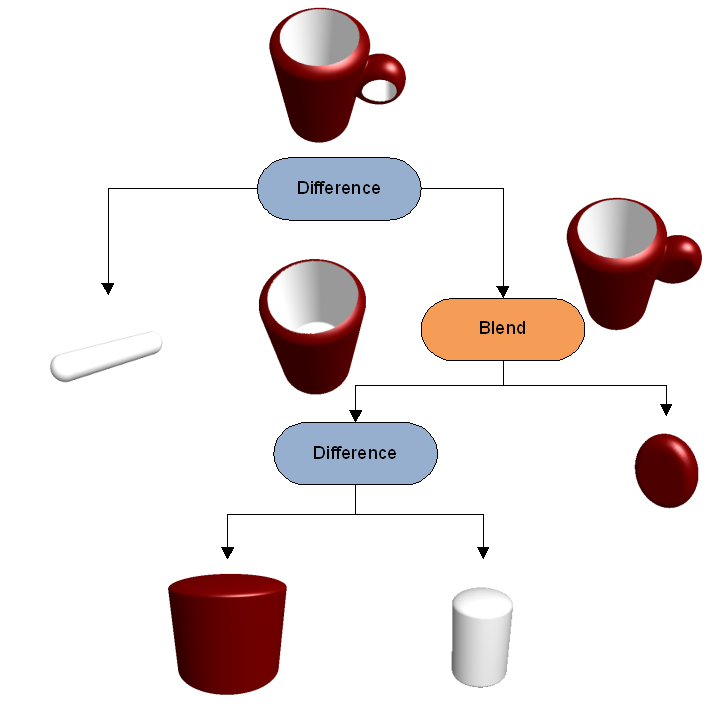
\includegraphics[width=1.0\linewidth]{figures/intro/CoffeeMugBlobTree}
  \caption{\blob structure of a coffee mug created with CSG and skeletal implicit primitives.}
  \label{fig:CoffeeMugBlobTree}
\end{figure}

%As the tree gets deeper and the number of primitives increase the computation 
For visualization purposes the \blob is queried numerous times to evaluate the field. As suggested in \cite{SWG2005} 
accelerating field computation will have a large impact on the overall surface extraction process. 

\section{Sweep Surfaces and Sketching}
Implicit primitives in our system are created from skeletons which are simple geometrical shapes such as points, line segments or 
polygons from which volumetric distance fields are created. In order to support more complex geometries \textit{Schmidt} \etal proposed the
implicit sweep objects technique where the 2D shape sketched by the user is sampled and an implicit approximation is created from 
the sample points \cite{Schmidtc}. This is done by fitting a thin-plate spline as a base shape to the sampled points using variational 
interpolation \cite{Turk1999}. One advantage of creating the base shape using variational interpolation is that the resulting implicit 
field is $C^2$ continuous, a property needed when the shape is involved in several blending operations \cite{barthe2004controllable}.

A continuous 2D scalar field is created from several field value samples $(\mathbf{m}_i, v_i)$, where $\mathbf{m}_i$ describes the 
position of the sample and $v_i$ is the desired field. The thin-plate spline used to create the variational 
implicit field $f_c(\mathbf{u})$ is defined in terms of these points weighted by corresponding coefficients $w_i$ combined with a polynomial 
$P(u) = c_1u_x +c_2u_y +c_3$.

\begin{equation}
f_c(\mathbf{u}) = \sum_{i \in N} w_i(\|\mathbf{u}-\mathbf{m}_i\|)^2ln(\|\mathbf{u}-\mathbf{m}_i\|)+P(\mathbf{u}) 
\label{eq:thinplatespline}
\end{equation}

The weights $w_i$ and coefficients $c_1$, $c_2$, and $c_3$ are found by solving a linear system defined by evaluating 
equation \ref{eq:thinplatespline} at each known solution $f_c(\mathbf{m}_i)=v_i$.
The resulting thin plate spline can then be used as the basis of several different primitives:

\begin{itemize}
 \item Inflated Objects
 \item Swept object along a trajectory
 \item Revolving object around axis
\end{itemize}

These sketched objects can then be used in the same way as the standard skeletal implicit primitives to create unique 3D shapes. Such 
unique shapes were not possible to create in previous collaborative environments, especially given the small memory footprint 
needed to transfer the information when using this technique.



%-------------------------------------------------------------------------
\section{Related Work}
\label{sec:relatedwork}

In the following we review the related work associated with the major contributions of our research. 
The surface extraction methods that attempted to enhance the performance of the 
sampling process on multi-core CPU processors are reviewed first. Some others attempted to exploit the processing 
power on the GPU and mapped the same problem to many-core processors. Later 
the previously proposed algorithms for cutting volumetric meshes and the application of this framework 
in a surgical simulation (Craniotomy) are studied. 


\subsection{Surface extraction methods}
Several methods for polygonization of implicit surfaces have been proposed which can be 
classified based on speed, accuracy of the output mesh or quality.  Comparing these methods in terms of performance reveals that space 
partitioning methods are the fastest and the most popular. The paper \cite{Wyvill1986} was the first to introduce a method for finding 
iso-surfaces using uniform space subdivision into cubic cells. A seed cell on the surface was found by starting at a vertex close to 
each primitive and evaluating the field at cell vertices along each of the three axes to find a surface crossing. Vertices inside the 
volume were classified as `hot' and `cold' outside. A hash table was used to keep track of processed cells to avoid redundant field 
evaluations and to avoid storing any cells that did not contain part of the surface. Only adjacent cells that share an intersecting edge 
with their parent were processed, and a second cubic subdivision served to reduce the number of primitives considered in each field evaluation. 
Ambiguous cases were ameliorated by taking another sample from the center of the face.
A similar method was later introduced as Marching Cubes in \cite{Lorensen1987}. The main difference between the two algorithms was that 
Lorenson \etal applied their method to discrete volume data instead of sampling a continuous function and in Lorenson's method
the space was completely partitioned into cubic voxels and all cubes were visited.

Bloomenthal showed that the ambiguous cases can be dealt with by subdividing cells into tetrahedra \cite{Bloomenthal1994a}, and also 
that a six tetrahedron subdivision was superior to subdividing into five \cite{guziec1995exploiting}. 
The fact that tetrahedral simplices have 4 vertices reduces the total number of configurations to 16 (or 3 by symmetry), however, the number of 
redundantly generated triangles as a result of this decomposition increases significantly. 
We will refer to marching cubes and tetrahedra, with MC and MT respectively throughout this chapter.

%4. Serial Ehancements to MT and MC
There have been many enhancements proposed for both MC and MT. Some gain advantage by classifying cubes according to different criteria
and surface edge intersection calculation and number of field function evaluations. 
For example, Dietrich \etal \cite{Dietrich2009}, did a statistical analysis of cube configurations in MC that are responsible for most 
of the degenerate triangles in the output mesh. Their algorithm avoids those cube configurations by inserting an extra vertex into the 
cell when generating triangles as was done in \cite{Wyvill1986} where an extra sample was taken.
This reduces the statistical occurrence of the problem.

Triquet \etal \cite{Triquet2003} enhanced MT by applying time-stamps on calculated values and using hash tables for retrieving them. They
also pre-computed surface vertices along crossing edges which are shared with adjacent voxels and referenced previously calculated
values to avoid re-evaluating them. This latter enhancement was also done in Bloomenthal's polygonizer \cite{Bloomenthal1994a}
and was a fairly common feature of implicit surface polygonizer's of the 1990s.

%5. Parallel Enhancements on CPU
Beside enhancing serial algorithms some attempts were made to increase the performance of MC by dividing the workload between
multiple CPUs or on a network grid of computers. Mackerras proposed an MIMD implementation of MC algorithm \cite{mackerras1992fast}. 
The bounding volume is divided into uniform blocks and each processor runs a serial implementation of MC on one or more blocks. They 
reported that because of efficient usage of cache their method showed a speed-up greater than the total number of physical
processors involved. Hansen and Hinker presented a parallel implementation of MC \cite{hansen1992massively}. They labeled each cube
with a virtual processor identifier to avoid complexities in communicating between processors, then each cube is processed
independently. They reported linear speed-up by increasing the number of physical processors. Their method spends constant time on
each processor regardless of the number of polygons in a cubic cell.

%6. GPU polygonizers
The advent of shader programs and GPGPU computing interested some to port serially computationally intensive programs to the GPU. 
Space partitioning methods like MC and MT are good candidates for these devices since each cell (either tetrahedra or
cube) can represent an independent volume to be processed on a separate SIMD core. 

%Kipfer and Westerman paper
Kipfer and Westermann proposed a GPU-accelerated Marching Tetrahedra algorithm that stores the topology of the
surface on the GPU \cite{Kipfer2005}. They used a span-space interval tree to cull tetrahedral elements that don't intersect with the 
surface. Caching edge-surface intersections helped them to avoid redundant calculations. For computing edge-surface intersections they used
linear interpolation for finding roots along each edge which is less accurate and degrades the quality of the output mesh.  

%Johansson paper
Johansson \etal accelerated iso-surface extraction using graphics hardware \cite{Johansson2006}. They stored MC cases on the GPU 
and used a vertex program to compute surface intersection points. They used a span-space data-structure similar to \cite{Cignoni1997} to
enhance the cell classification phase in MC. Their method shows a speedup order of 13 over the naive algorithm.  


% DirectX$^{\textregistered}$ 10 is not needed
Tatarchuk \etal presented an iso-surface extraction algorithm implemented using DirectX \cite{Tatarchuk2008}. They used graphics 
hardware to visualize medical data. They maximized utilization of SIMD units on the GPU by separating their polygonization (which is a 
hybrid of marching cubes and marching tetrahedra) into two phases: Fast cube tetrahedralization and a marching tetrahedra pass. Each input 
voxel position is dynamically computed in the vertex shader, then they used the geometry shader and stream-out features of DirectX 10 to 
tessellate voxels into six tetrahedra spanning the voxel cube. However their method is limited to medical volume datasets.

%Parallel Polygonization
An adaptive parallel polygonization method is proposed by Yang \etal \cite{Yang2010}. They enhanced the Araujo's method 
\cite{Rodriguesdearaujo2005} by dividing the bounding box of the model into eight parts and then processing them in parallel.
For each part, their method find a seed point on the surface and increasingly expand it to form a 
local mesh for the part by using the surface tracking approach. Using local curvature of the implicit 
surface, their method produces triangles of varying sizes. However, their method is not scalable since 
it can not guarantee finding a seed point per each sub box in case the number of sub boxes increases. 
They reported very slow rendering times even for the simple models that they have tested their system with. 


In a similar work Knoll \etal \cite{Knoll2007} proposed interactive raytracing of arbitrary implicits with 
SIMD interval arithmetic. They used SSE instructions for fast computation of interval arithmetic 
and ray traversal algorithm. However, their method is restricted to static implicit functions and 
algebraic surfaces.

None of the proposed methods above used a modelling framework to define their input data in a hierarchical structure similar to 
the \blobns. Their method is either limited to volume data or an algebraic implicit function to represent the underlying volume. 
In a closely related work, Schmidt \etal \cite{SWG2005} used a field caching mechanism inside the \blob to perform fast potential field 
reconstruction without traversing the entire tree. They used a trilinear reconstruction filter for field value and a triquaratic filter
for gradient interpolation. They evaluated cache efficiency by polygonizing a \blob model once using cache nodes and the other time 
without. They reported up to 16 times speedup for polygonizing a model with different resolutions. However, their method is not scalable since 
the cache nodes cannot be updated from different processing threads without using locking
mechanisms or a data race condition can occur. 

\subsection{GPU-Accelerated rendering of implicits}
GPU accelerated rendering techniques has been the topic of interest for the graphics community in the past two decades.
Several GPU-accelerated algorithms have been proposed for fast triangulation and rendering of iso-surfaces that are defined by
volume data-sets, algebraic surfaces and radial-basis functions. In this section we will review the most related works.

Chochl{\'i}k \etal proposed a GPU accelerated polygonization algorithm for dynamically changing implicit surfaces \cite{chochlik2012gpu}. 
Their method is based on the marching tetrahedra (MT) algorithm. The model is partitioned into cubic cells first and then each cell is 
subdivided into 6 tetrahedra to be further processed using the GPU geometry shading stage. The vertices are marked inside if their 
associated field is above zero and outside otherwise. A configuration index is computed per each tetrahedra based on the inside/outside 
vertices. The triangle mesh is produced which is shaded using the fragment shader stage. No further analysis has been made on the performance 
of their algorithm and the input models are limited to time varying simple algebraic surfaces. The used a linear interpolation root finding
method which produces low quality output. 

Buatois \etal proposed a GPU accelerated iso-surface extraction method based on MT, similar to Chochl{\'i}k \etal \cite{Buatois2006}. The 
texture memory to transfer the position and field values of the grid vertices. They presented an analysis of the performance of their algorithm
using a fluid simulation volume data-set. They reported that excessive texture fetches can be a bottleneck in the performance of their method.


Tatarchuk \etal proposed a GPU iso-surface extraction algorithm which is a hybrid of marching cubes and marching tetrahedra \cite{Tatarchuk2007}. 
They start by voxelizing an implicit grid into discrete cube cells and then convert that to a tetrahedral representation. They implemented an MT 
algorithm on geometry shader stage of DirectX10 API. For root finding method they fitted a parabola along the intersecting edges and evaluated a 
quadratic equation which produces a better approximation. They tested their system using the visible human volume data-set. Their method
is limited to static volume datasets and is not usable in a data-driven setting where the topology of the underlying model changes. 

With modern hardware and fast GPUs, ray tracing of implicit surfaces is the subject of much research. Knoll \etal \cite{Knoll2009} presented 
CPU and GPU algorithms that can achieve interactive visualization for common algebraic surfaces. The surfaces used in by Knoll \etal are not 
arbitrary implicit models but surfaces generated using traditional kernels or functions. Similar surfaces are presented by Singh and Narayanan
for real-time ray tracing of implicit surfaces using the GPU \cite{singh2010real}. 


Kipfer and Westermann \cite{Kipfer2005} accelerated rendering of implicit surfaces by avoiding redundant computation of edge surface intersections. 
Our method also employs this feature to reduce the overhead. They also use features of the GPU to reformulate the iso-surface identification and reduces 
numerical computations and memory access operations. They used a span-space data-structure to avoid processing non surface intersecting elements.

Kanai \etal \cite{Kanai2006a} proposed a rendering method for sparse low-degree implicit surfaces (SLIM) using ray casting approach. The ray and IS intersection
test has been carried out on the fragment processing stage. They employed level of detail rendering and view frustum culling to speedup the rendering. 
The coefficients for the IS are passed in using textures. They reported high quality and interactive rates for several models. The large number of processed
fragments is the bottleneck in this process and models with lower number of nodes could be rendered slower than more complex models that cover less fragments.
Although Kanai \etal's work is data-driven but the increasing cost of fragment processing is the main bottleneck in their system. Also since they are not
producing any mesh the computations will be lost after rendering.

\subsection{Volume mesh cutting}
A number of approaches has been proposed by the computer graphics community to enable cutting of deformable and rigid models. 
Except for a few methods most of them use tetrahedral meshes for the volumetric mesh representation. 
Bielser \etal performed an adaptive refinement of the tetrahedral elements cut by a virtual scalpel \cite{Bielser1999}.
In another work Bielser \etal presented a progressive approach to cutting \cite{Bielser2003}, where the decomposition of 
a tetrahedron is changed depending on the movement of the cutting tool inside an element. However, the approach is highly 
non-trivial to implement and also poses some stability problems due to badly-shaped elements.

Mor \etal tried to reduce the number of sub-elements created while cutting tetrahedral meshes \cite{Mor2000}.
One of the major issues in cutting is the creation of ill-shaped elements i.e. skinny elements, which can adversely affect the
performance and stability of the system solver. Some work attempted to avoid such elements via mesh alignment techniques 
\cite{Nienhuys2001b, Steinemann2006}. Other methods tried to solve the issue by removing them completely which resulted in 
volume loss and jagged lines along the cut surface. 

 
Wu \etal \cite{Wu2011} proposed an algorithm for 3D mesh cutting using a combination of the adaptive octree refinement with an iterative composite
element hierarchy to enable simulating high-resolution cuts with a small number of degrees of freedom (DOFs). 
They used the dual contouring method \cite{Ju2002} to keep the sharp creases along the cut. Due to the high computational cost and naive implementation 
their method is not scalable and has yet to become an interactive cutting approach.

In a closely related work Courtecuisse \etal presented a soft-tissue cutting system with haptic 
feedback \cite{Courtecuisse2010}. Their cutting strategy follows Mor \etal  \cite{Mor2000} work and 
suffers from jagged lines along the cut surface as shown in their examples of a laparoscopic hepatecotomy.
Progressive cutting, a feature that enables cutting the volume elements as soon as they become in contact with 
the scalpel, is not supported in their system and as most of the other works in this area they produce too many
new nodes when subdividing cut elements.

Jerabkova \etal proposed a solution to the ill-shaped elements problem by using hexahedral elements instead of 
tetrahedra \cite{Jerabkova2010}. Their approach relies on fine-level voxels to model object surface and simulate cutting. 
The volume data requires more memory space than traditional, surface-based models. Cutting is performed by
removing voxels. For sufficiently small voxels this typically remains unnoticeable but it may result in 
significant volume loss in case of a large number of cuts. 

Jin \etal proposed a meshless total Lagrangian adaptive dynamic relaxation cutting algorithm to predict the steady-state 
responses of soft tissue \cite{Jin2013}. A cloud of points is used for discretization and approximation of the deformation 
field within the continuum without generation of finite element meshes. They didn't report any performance measurements 
and the quality of the cuts could not be verified with the simple truth cube model they reported in their paper.

Sifakis \etal \cite{Sifakis2007} proposed a geometric algorithm for placing cracks and incisions on 
tetrahedralized deformable objects. Their method is similar to the virtual node algorithm in that they avoid 
sliver elements and their associated stringent timestep restrictions. Producing ill-conditioned triangles on 
the material surface can have a negative effect on collision handling specially in case of a self collision.
Also in their system a cut that partially intersects a tetrahedron without separating it into disconnected 
fragments will not allow the material to separate within that embedding tetrahedron.

Steinemann \etal \cite{Steinemann} created a hysteroscopy simulator and minimized the number of added elements 
after a tetrahedral subdivision by cutting along existing edges and faces. The problem with their system is that
the result of the cutting is produced only after it has been completed and this leads to a delay in the system. 
Unfortunately they didn't report any performance statistics of their algorithm. 

In the following sections we provide an overview of the system and the data structures involved in the process 
and our cutting algorithm. The chapter is concluded by the analysis of the simulation results.

\subsection{Applications in Surgical Simulation}
Abe \etal fabricated plastic skull models of seven individual patients by stereolithography from three-dimensional
data based on computed tomography (CT) bone images \cite{Abe1998}. Surgical approaches and areas of craniotomy were 
evaluated using the fabricated skull models. They reported a better understanding of anatomic relationships, preoperative
evaluation of the proposed procedure and improved educational experiences for the residents and medical staff as the benefits of 
their system. They also reported that the time and cost of making such models are the main disadvantages of using them.

Wong \etal loaded patient specific CT scans of cranial bone and CT angiography of intracranial circulation
into the Dextroscope workstation supplied by Volume Interactions Pte. Ltd \cite{Wong2007}. They showed various 
use-cases of the zoom, rotate, move and crop functions of the Dextroscope to visualize various angles of 
positioning the craniotomy. However, their system does not provide a physically-based simulation of the procedure. 

Stadie \etal performed a study on the effectiveness of virtual reality systems for placing the craniotomies 
in minimally invasive procedures \cite{Stadie2011}.  They used the Dextroscope and RadioDexter workstations 
supplied by Volume Interactions Pte. Ltd. to visualize and annotate the 3D VR models. 
Those systems are also used to measure the curvilinear distances of the proposed craniotomy centers on the 
patients skull model but they can not perform a cutting procedure on the input VR models.



\setlength{\unitlength}{\savedunitlength}
